\subsection{Thiết kế ý niệm}

\subsubsection{Mô hình kho dữ liệu}\label{sec:mohinhkho}

Dựa trên phạm vi đề tài đã xác định ở mục~\ref{sec:phamvi}, trong ba mô hình kho dữ liệu: Enterprise Data Warehouse -- EDW, Data Mart và Virtual Data Warehouse \cite{han}, đề tài được xây dựng theo mô hình \textit{Data Mart} trực tiếp từ bộ dữ liệu nguồn có sẵn. Lựa chọn này xuất phát từ các lý do sau:

\begin{itemize}
\item Phạm vi dữ liệu tập trung vào một mảng nghiệp vụ: Dữ liệu nguồn chỉ bao gồm hoạt động bán hàng và giao nhận trên sàn, không có dữ liệu về các phòng bàn khác như marketing hay nhân sự. Trong khi đó, EDW được thiết kế để tích hợp dữ liệu của toàn bộ tổ chức nên không phù hợp với phạm vi của đề tài.
\item Nguồn dữ liệu đơn giản: Toàn bộ dữ liệu đến từ một nguồn duy nhất là 9 tập tin CSV của Olist (Bảng~\ref{tab:nguon}), do đó không cần đến quy trình tích hợp phức tạp giữa nhiều hệ thống như một EDW.
\item Phù hợp với mô hình đa chiều: Data Mart thường được thiết kế theo star schema hoặc snowflake schema, phù hợp với yêu cầu thiết kế kho dữ liệu theo mô hình đa chiều.
\end{itemize}

Mô hình Virtual Data Warehouse không được lựa chọn vì mô hình này không lưu trữ dữ liệu đã qua xử lý, trong khi dữ liệu nguồn có nhiều vấn đề cần làm sạch trước khi sử dụng (Bảng~\ref{tab:chatluong}) và mô hình này có hiệu năng truy vấn thấp hơn khi làm việc với dữ liệu lớn.

Mặc dù hệ thống phục vụ nhiều nhóm người dùng như ban điều hành, quản lý vận hành và bộ phận chăm sóc khách hàng, các nhóm này đều khai thác cùng một mảng dữ liệu là \textit{đơn hàng} của sàn. Hạn chế của Data Mart là có thể trở thành nguồn dữ liệu tách biệt khi tổ chức bổ sung thêm các nguồn dữ liệu khác. Để khắc phục, nhóm thiết kế các chiều thời gian, địa lý và sản phẩm theo dạng chiều đồng nhất (conformed dimensions) \cite{kimball}, tức có cùng cấu trúc và cách mã hóa để các Data Mart khác có thể sử dụng lại, tạo điều kiện tích hợp Data Mart vào một kho dữ liệu lớn hơn trong tương lai.

\subsubsection{Hướng tiếp cận xây dựng mô hình}

Nhóm lựa chọn hướng tiếp cận \textit{Bottom-up} vì đây là hướng phù hợp với mô hình Data Mart đã chọn ở mục trước. Lựa chọn này xuất phát từ các lý do sau:

\begin{itemize}
\item Nhất quán với mô hình Data Mart: Hướng Bottom-up lấy Data Mart làm điểm khởi đầu.
\item Triển khai nhanh và tiết kiệm chi phí: Hướng Bottom-up tập trung vào một nhu cầu cụ thể nên có thể đưa vào sử dụng sớm, với chi phí và thời gian phát triển thấp hơn.
\item Đáp ứng trực tiếp nhu cầu phân tích: Data Mart được xây dựng xoay quanh các chỉ số và quyết định đã xác định ở Bảng~\ref{tab:kpi} và Bảng~\ref{tab:quyetdinh}, giúp người dùng khai thác được kết quả ngay.
\item Phù hợp với quy mô đề tài: Hướng Bottom-up phù hợp với các tổ chức vừa và nhỏ có nhu cầu phân tích cụ thể và nguồn lực hạn chế.
\end{itemize}

% Hướng Top-down không phù hợp vì đòi hỏi xây dựng trước một EDW với thời gian phát triển dài, chi phí lớn và cần dữ liệu của toàn bộ tổ chức, trong khi dữ liệu nguồn chỉ có một mảng nghiệp vụ. Hướng Hybrid cũng không phù hợp vì yêu cầu phối hợp đồng thời giữa EDW và các Data Mart.

Áp dụng hướng Bottom-up, đề tài được triển khai theo các bước sau:

\begin{enumerate}
\item Xây dựng Data Mart cho mảng bán hàng và giao nhận của sàn, phục vụ các nhu cầu phân tích về doanh thu, giao hàng, mức độ hài lòng và hiệu quả người bán.
\item Xây dựng quy trình ETL để trích xuất, làm sạch và nạp dữ liệu từ các tập tin nguồn Olist vào Data Mart.
\item Xây dựng các công cụ báo cáo và phân tích OLAP trên Data Mart để phục vụ người dùng.
\item Khi có thêm nguồn dữ liệu mới, xây dựng thêm các Data Mart khác và tích hợp với Data Mart hiện tại thông qua các chiều đồng nhất.
\end{enumerate}

Hạn chế của hướng Bottom-up là các Data Mart có thể trở nên rời rạc và khó tích hợp nếu không được thiết kế thống nhất. Như đã trình bày ở mục~\ref{sec:mohinhkho}, nhóm khắc phục hạn chế này bằng cách thiết kế các chiều thời gian, địa lý và sản phẩm theo dạng chiều đồng nhất ngay từ đầu.



\subsubsection{Kiến trúc tổng thể của hệ thống}\label{sec:kientruc}

Hệ thống được thiết kế theo kiến trúc ba tầng của kho dữ liệu. Kiến trúc này tách biệt việc lưu trữ, xử lý phân tích và trình bày dữ liệu, giúp mỗi tầng có thể được phát triển và mở rộng độc lập. Hình~\ref{fig:kientruc} trình bày kiến trúc tổng thể của hệ thống.

\begin{figure}[H]
\centering
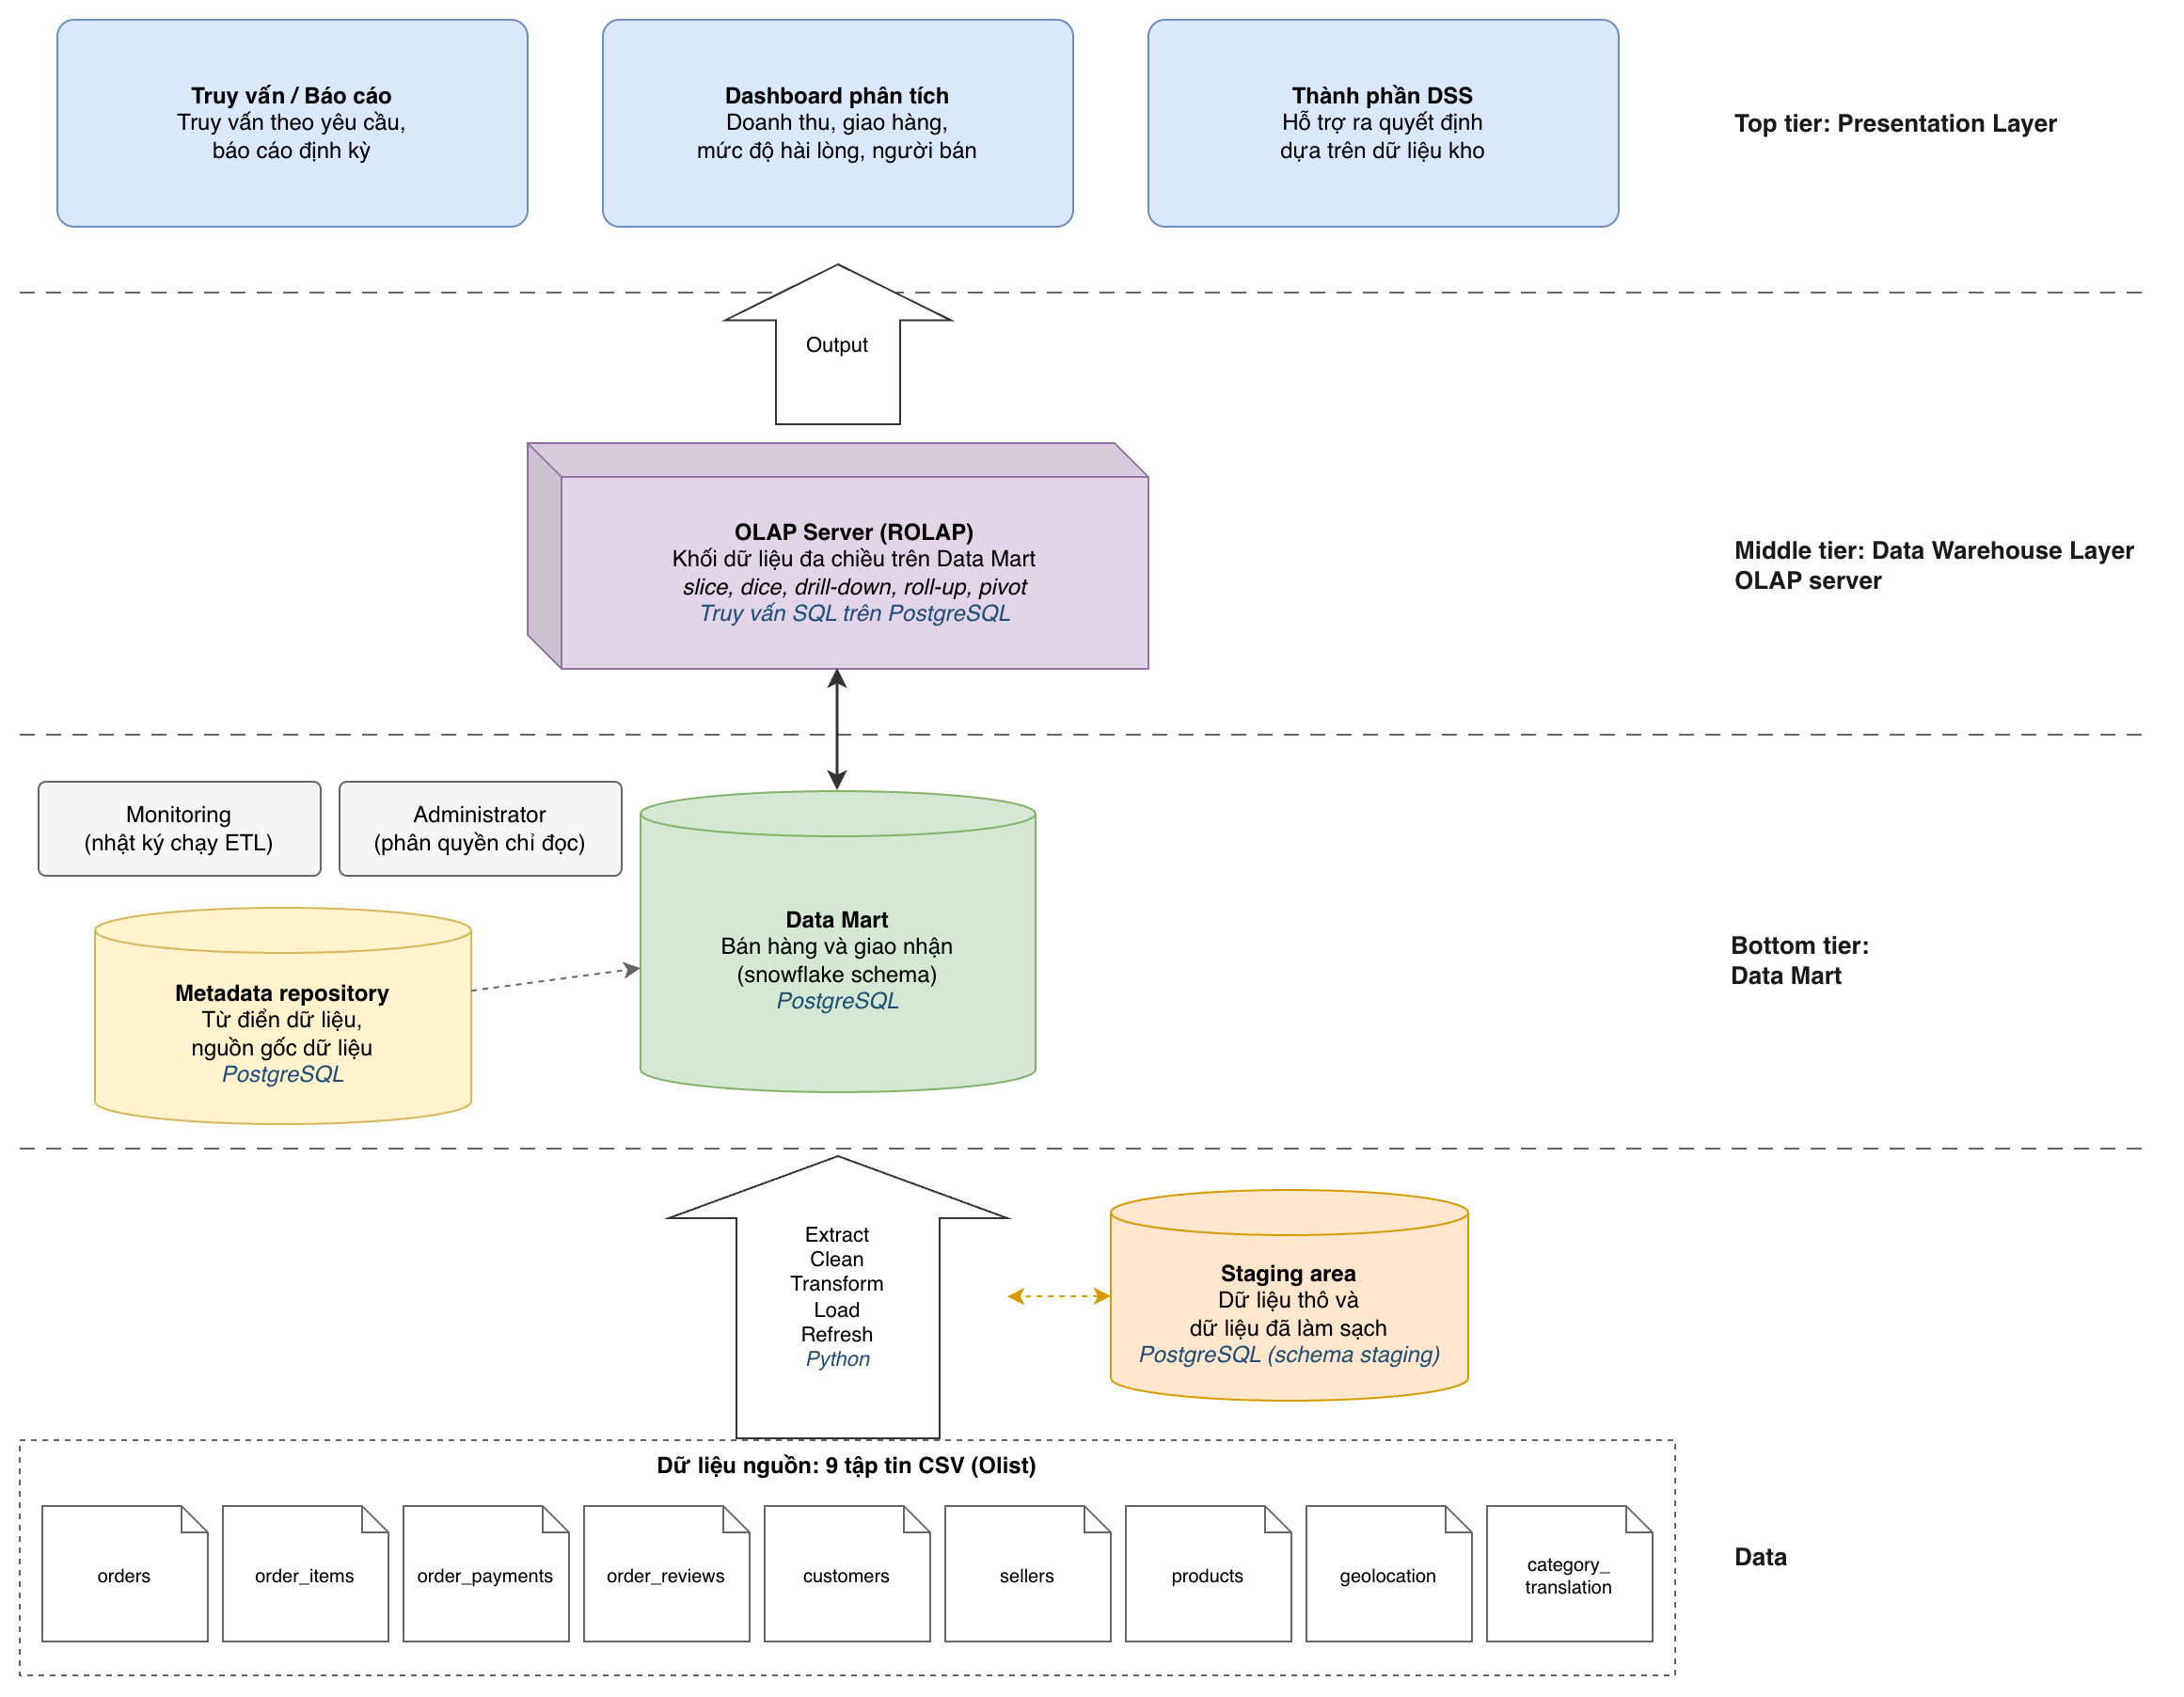
\includegraphics[width=\linewidth]{Pictures/kien-truc.png}
\caption{Sơ đồ kiến trúc ba tầng của hệ thống}
\label{fig:kientruc}
\end{figure}

Các thành phần của kiến trúc được mô tả như sau:

\begin{itemize}
\item Dữ liệu nguồn (Data): Gồm 9 tập tin CSV của bộ dữ liệu Olist (Bảng~\ref{tab:nguon}). Dữ liệu được đưa vào kho thông qua quy trình ETL viết bằng Python, gồm các bước trích xuất (Extract), làm sạch (Clean), biến đổi (Transform), nạp (Load) và làm mới (Refresh). Trong quá trình này, dữ liệu được lưu tạm tại khu vực staging, là một schema riêng trong PostgreSQL, chứa cả dữ liệu thô và dữ liệu đã làm sạch. Đây là nơi xử lý các vấn đề chất lượng dữ liệu đã nêu ở Bảng~\ref{tab:chatluong} trước khi nạp vào Data Mart.
\item Tầng dưới (Bottom tier) -- Data Mart: Là nơi lưu trữ dữ liệu đã được tích hợp, gồm Data Mart bán hàng và giao nhận được tổ chức theo snowflake schema trên PostgreSQL. Đi kèm Data Mart là kho metadata (metadata repository) lưu từ điển dữ liệu và nguồn gốc dữ liệu, cùng với hai chức năng giám sát (Monitoring) qua nhật ký chạy ETL và quản trị (Administrator) qua phân quyền chỉ đọc cho người dùng phân tích.
\item Tầng giữa (Middle tier) -- OLAP server: Nhóm sử dụng mô hình ROLAP, trong đó khối dữ liệu đa chiều được xây dựng trực tiếp trên Data Mart và các phép toán \texttt{slice}, \texttt{dice}, \texttt{drill-down}, \texttt{roll-up}, \texttt{pivot} được thực hiện bằng truy vấn SQL trên PostgreSQL. Mô hình này phù hợp vì dữ liệu đã được lưu trong cơ sở dữ liệu quan hệ và quy mô dữ liệu cho phép tổng hợp trực tiếp với thời gian phản hồi chấp nhận được.
\item Tầng trên (Top tier) -- Presentation Layer: Gồm các công cụ truy vấn và báo cáo, dashboard phân tích về doanh thu, giao hàng, mức độ hài lòng và hiệu quả người bán, cùng với thành phần hệ hỗ trợ quyết định (DSS) khai thác dữ liệu từ kho.
\end{itemize}

%% update in future when change the technology stack
Về công nghệ, nhóm sử dụng Python để xây dựng quy trình ETL và PostgreSQL để lưu trữ khu vực staging, Data Mart và metadata. Việc sử dụng một hệ quản trị cơ sở dữ liệu duy nhất cho các thành phần lưu trữ giúp hệ thống đơn giản, dễ triển khai và dễ bảo trì, phù hợp với quy mô của bài tập lớn.
